\subsubsection{Die schwache Form am Beispiel des Stabes}

\begin{figure}[!htbp]
\centering
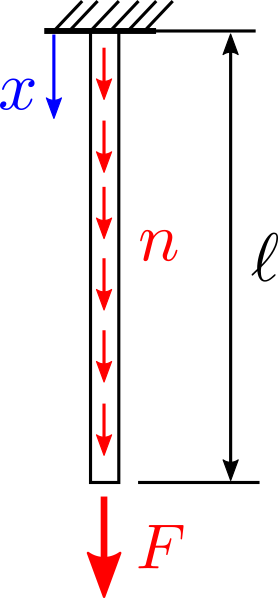
\includegraphics[width=0.25\linewidth]{files/Stab-8a25db6f500d6b4900b1c83a048e0388.png}
\caption[]{Stab unter Eigengewicht und externer Kraft.}
\label{stab_fig}
\end{figure}

Auch hier beginnen wir mit der starken Form der Differentialgleichung:
\begin{equation}
\label{stabdglsimple_2}
 {EA} u^{\prime \prime} =  - {n(x)} A \; ,
\end{equation}

\begin{framed}
\textbf{Analytische Lösung}\\
Die analytische Lösung erhalten wir durch zweifache Integration und Einsetzen der Randbedingungen:
\begin{equation}
u(x) = \left( \frac{F}{EA} + \frac{n \ell}{E}\right)\cdot x - \frac{1}{2} \frac{n}{E} x^2 \; .
\end{equation}
Die Schnittkraft $N$ berechnet sich wie folgt:
\begin{equation}
N(x) = F + n A (\ell-x).
\end{equation}
\end{framed}

Zur Herleitung der Finite-Elemente-Form multiplizieren wir die starke Form mit der Testfunktion $\delta u$ und integrieren die Gleichung über das Gebiet:
\begin{equation}
\label{stabdglsimple_weak}
 \int_{0}^{\ell} \delta u u^{\prime \prime} \dx = \int_{0}^{\ell} - \delta u \frac{n(x)}{EA} \dx\; .
\end{equation}
Der Ausdruck auf der linken Seite wird umgeformt zu:
\begin{equation}
\label{stabdglsimple_product}
 \int_{0}^{\ell} \delta u u^{\prime \prime} \dx = \int_{0}^{\ell} \left(\delta u u^{\prime}\right)^{\prime} - \delta u^{\prime}  u^{\prime}  \dx\; .
\end{equation}

Ersetzen wir nun $\delta u^{\prime}=\delta \e$ und $u^{\prime}=\e$ und setzen die obige Produktregel in Gleichung (\ref{stabdglsimple_weak}), so erhalten wir:
\begin{align}
 \int_{0}^{\ell} \delta \e \cdot E\e \, A \dx & = \left[\delta u \cdot \sigma A \right]_0^{\ell} + \int_0^{\ell} \delta u \cdot n(x) \dx\;  \\
 & = \left[ \delta u(\ell) \cdot F + \delta u(0) \cdot 0\right]+ \int_0^{\ell} \delta u \cdot n(x) \dx\; .
 \end{align}

\paragraph{Das Verfahren von Ritz}

Als Einführung in die Finite-Elemente-Methoden beginnen wir mit dem Verfahren, welches von Walter Ritz (1878 - 1909) eingeführt wurde. Dies fu$\beta$t auf dem Prinzip der virtuellen Arbeit, formuliert als $\delta U - \delta W = 0$, wobei $\delta U$ für die Arbeit der inneren Kräfte und $\delta W$ für die der äu$\beta$eren Kräfte steht. Für einen einfachen Stab ergibt sich die obige schwache Form (\ref{stabdglsimple_weak2}).

Der nächste Schritt ist die Aufstellung einer Näherungslösung $u_h$ für das Verschiebungsfeld $u$, zum Beispiel durch eine quadratische Funktion:

\begin{equation}
u_h(x) = a_0 + a_1 x + a_2 x^2,
\end{equation}

wobei die Koeffizienten $a_i$ durch Minimierung der virtuellen Arbeit ermittelt werden müssen. Diese Parameter müssen gleichzeitig kinematische Verträglichkeit garantieren und somit die geometrischen Randbedingungen einhalten. Aus $u(0) = 0$ ergibt sich dann $a_0 = 0$. Die benötigte Ableitung des Näherungsansatzes lautet daher:

\begin{equation}
\e = u^{\prime} = a_1 + 2a_2 x.
\end{equation}

Die Variationen dieses Ansatzes werden durch Variieren der Koeffizienten gebildet:

\begin{equation}
\delta u(x) = \delta a_1 x + \delta a_2 x^2
\end{equation}

und

\begin{equation}
\delta \e= \delta a_1 + 2 \delta a_2 x.
\end{equation}

Eingesetzt in das Prinzip der virtuellen Arbeit führt es zu:

\begin{equation}
EA \int_0^{\ell} (\delta a_1 + 2 \delta a_2 x) (a_1 +2 a_2 x) \dx = F (a_1 \ell +a_2 \ell^2) + \int_0^{\ell} (\delta a_1 x + \delta a_2 x^2) n A \dx \; .
\end{equation}

Nach Integration und Herausziehen der Variationen resultiert daraus:

\begin{equation}
\delta a_1\left[EA \ell (a_1 + a_2 \ell) - \frac{1}{2} n A \ell^2 - F \ell\right] + \delta a_2 \left[EA\ell^2(a_1 + \frac{4}{3}a_2\ell) - \frac{1}{3}nA\ell^3 - F\ell^2\right] = 0.
\end{equation}

Da die Variationen beliebig sind, müssen die in eckigen Klammern stehenden Terme jeweils null sein. Daraus folgt ein lineares Gleichungssystem zur Bestimmung der Koeffizienten, das gelöst wird als:

\begin{equation}
a_1 = \frac{F}{EA} + \frac{n \ell}{E} \qquad \text{und} \qquad  a_2 = -\frac{n}{2E}.
\end{equation}

Somit erhalten wir als Näherungslösung für diesen Fall:

\begin{equation}
u_h(x) = \left(\frac{F}{EA} + \frac{n \ell}{E}\right)x - \left(\frac{n}{2E}\right)x^2.
\end{equation}

Man kann leicht erkennen, dass mit diesem quadratischen Ansatz die analytische Lösung der Differentialgleichung rekonstruiert werden konnte.

\begin{framed}
\textbf{Problem}\\
Ein Problem beim Ritz'schen Verfahren ist die Wahl der Ansatzfunktion. Diese muss die Randbedingungen erfüllen und die Stetigkeitsanforderungen der schwachen Form. Für komplexere Probleme ist die Wahl der Ansatzfunktion nicht trivial und oft auch nicht möglich.
\end{framed}

%  -+-+-+-+-+-+-AI-SPLIT

\paragraph{Finite Elemente Formulierung für den Stab}

\subparagraph{Diskretisierung der schwachen Form}

\begin{figure}[!htbp]
\centering
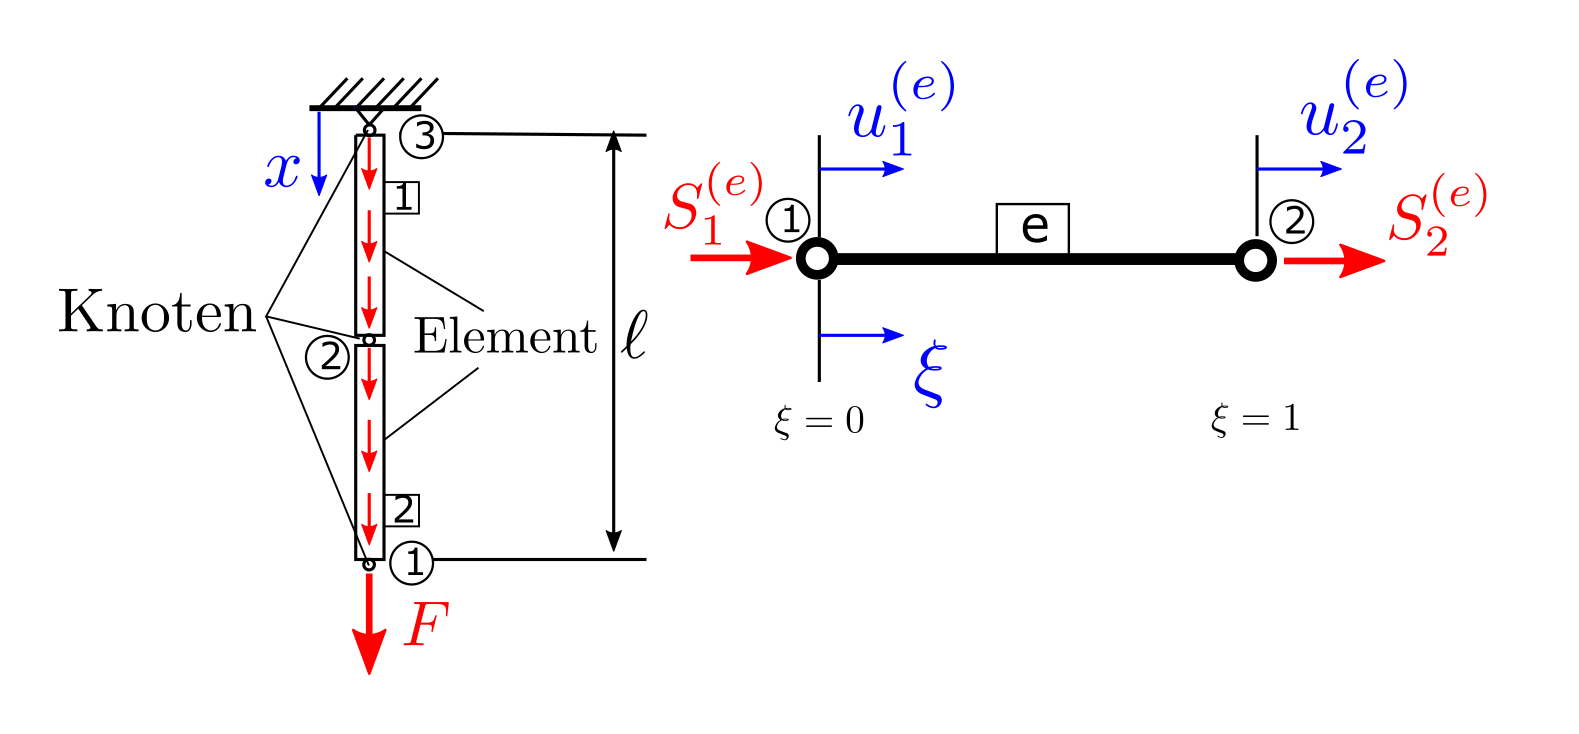
\includegraphics[width=0.75\linewidth]{files/Stab_element-be352cad5b74b55eb9e4829b97d1c026.png}
\caption[]{Stab unter Eigengewicht und externer Kraft mit Stabelementen diskretisiert.}
\label{stabelement}
\end{figure}

Im vorangegangenen Abschnitt haben wir die Effektivität des Prinzips der virtuellen Arbeit in Kombination mit dem Ritz'schen Verfahren untersucht. Es erweist sich jedoch oft als schwierig, einen angemessenen Näherungsansatz für komplexe Strukturen zu finden, die einer vielschichtigen Belastung ausgesetzt sind. Die Finite-Elemente-Methode (FEM) löst dieses Problem, indem sie einfache Ansatzfunktionen auf überschaubaren Teilbereichen -- den sogenannten finiten Elementen -- anwendet und diese dann systematisch für das gesamte Gebiet integriert.

Als Beispiel hierfür dient die im Bild Figure~\ref{stabelement} dargestellte Diskretisierung eines Stabes mit der Gesamtlänge $\ell$, der in zwei finite Elemente mit jeweils der Länge $l_i = \frac{\ell}{2}$ unterteilt wird.

\begin{framed}
\textbf{Allgemeines zu Finiten Elementen}\\
Ein finites Element besteht in dem vorliegenden Beispiel aus 2 Knoten. Sowohl die Knoten als auch die Elemente werden im Allgemeinen nummeriert, damit man sie eindeutig ansprechen kann. Im Bild sind die Elementnummern in den rechteckigen Kästen neben dem Element eingetragen. Die Knotennummern sind in den Kreisen neben den Knoten dargestellt. Die Knoten sind die Träger der primären Feldvariablen (hier: Verschiebung $u$), und das Ziel der Finite-Elemente-Berechnung ist die Bestimmung der primären Variablen, auch Freiheitsgrade (englisch: Degree of freedom \textbf{Dof}) an den Knoten. Im Bild Figure~\ref{stabelement} auf der rechten Seite ist ein einzelnes Stabelement dargestellt. Das Stabelement hat 2 lokale Knoten, und um die Verschiebung an diesen Knoten eindeutig zuzuordnen, verwenden wir die Notation:

$u_1^{e} \text{ Verschiebung } u \text{ am lokalen Knoten 1 von Element } e$

$u_2^{e} \text{ Verschiebung } u \text{ am lokalen Knoten 2 von Element } e$
\end{framed}

Auf diesen Elementen werden dann einfache Ansatzfunktionen verwendet, welche eine lineare Approximation des Verschiebungsfeldes darstellen:

\begin{align}
 N_1(\xi) & = (1-\xi) \qquad N_2(\xi)= \xi  \\
 u_h(\xi) & = N_1(\xi) u_1^{(e)}+ N_2(\xi) u_2^{(e)} \\
 u_h(\xi) & = \sum_{I=1}^2 N_I(\xi) u_I^{(e)}
 \end{align}

Hierbei wurde das lokale Koordinatensystem $\xi = \frac{x}{\ell_e} \; \in \; [0,1]$  eingeführt, damit der gewählte Ansatz für alle Stabelemente, unabhängig von der Stablänge $\ell_e$, gültig ist. In der Matrixschreibweise erhält man für den Ausdruck (\ref{LinearDisplacementAnsatz}):

\begin{align}
  u_h(\xi) & = \underbrace{\begin{bmatrix} (1-\xi) & \xi \end{bmatrix}}_{\bm{N}\T} \underbrace{\begin{bmatrix} u_1^{(e)} \\ u_2^{(e)}\end{bmatrix}}_{\bm{u}^{(e)}} = \bm{N}\T \bm{u}^{(e)}
 \end{align}

Zur Berechnung des Prinzips der virtuellen Verrückungen bzw. der schwachen Form wird zusätzlich die Ableitung des Ansatzes für $u_h$ benötigt. Diese repräsentiert die Dehnung des Stabes $\e = \Dd{u}{x}$. Da der Ansatz über die normalisierte Koordinate $\xi$ bestimmt wurde, berechnet sich die Ableitung über die Kettenregel:

\begin{equation}
\e_h = \Dd{u_h}{x} = \Dd{u_h}{\xi} \underbrace{\Dd{\xi}{x}}_{\frac{1}{\ell_e}} = \frac{1}{\ell_e} \begin{bmatrix} -1 & 1 \end{bmatrix} \begin{bmatrix} u_1^{(e)} \\ u_2^{(e)}\end{bmatrix}
\end{equation}

Für die Variation $\delta u$ und $\delta \e$ wählen wir den gleichen Ansatz:

\begin{equation}
\delta u_h = \begin{bmatrix}  (1-\xi) & \xi \end{bmatrix} \begin{bmatrix} \delta u_1^{(e)} \\ \delta u_2^{(e)}\end{bmatrix} \qquad \delta \e_h = \frac{1}{\ell_e} \begin{bmatrix} -1 & 1 \end{bmatrix} \begin{bmatrix} \delta u_1^{(e)} \\ \delta u_2^{(e)}\end{bmatrix}
\end{equation}

Betrachten wir nun das Prinzip der virtuellen Verrückungen in Gleichung (\ref{stabdglsimple_weak2}):

\begin{align}
 \textcolor{green}{\int_{0}^{\ell} \delta \e \cdot E\e \, A \dx} -\textcolor{red} {\int_0^{\ell} \delta u \cdot n A \dx} - \textcolor{blue}{\delta u(\ell) \cdot F} = 0\; 
 \end{align}

Setzen wir hier unseren gewählten Ansatz für $u$, $\e$, $\delta u$ und $\delta \e$ ein, dann erhalten wir die folgende Gleichung:

\begin{align}
 \textcolor{green}{\int_{0}^{1} \frac{1}{\ell_e} \begin{bmatrix} -1 & 1 \end{bmatrix} \begin{bmatrix} \delta u_1^{(e)} \\ \delta u_2^{(e)}\end{bmatrix}  EA \frac{1}{\ell_e} \begin{bmatrix} -1 & 1 \end{bmatrix} \begin{bmatrix} u_1^{(e)} \\ u_2^{(e)}\end{bmatrix}   \underbrace{\ell_e \d \xi}_{\dx}} \\
 - \textcolor{red}{\int_0^{1} \begin{bmatrix} (1-\xi) & \xi \end{bmatrix} \begin{bmatrix} \delta u_1^{(e)} \\ \delta u_2^{(e)}\end{bmatrix}  n A \ell_e \d \xi} - \textcolor{blue}{\begin{bmatrix} \delta u_1^{(e)} & \delta u_2^{(e)}\end{bmatrix} \begin{bmatrix} S_1^{(e)} \\ S_2^{(e)} \end{bmatrix}}  = 0\; 
\end{align}
%  -+-+-+-+-+-+-AI-SPLIT

Die Variation der Knotenverschiebung $\delta u_I$ und die Knotenverschiebung $u_I$ sind nicht abhängig von $\xi$ und können somit aus dem Integranden herausgezogen werden:

\begin{align}
 \begin{bmatrix} \delta u_1^{(e)} & \delta u_2^{(e)}\end{bmatrix}\left\{ \textcolor{green}{   \int_{0}^{1} EA \frac{1}{\ell_e} \begin{bmatrix} 1 & -1 \\ -1 & 1\end{bmatrix}  \d \xi \begin{bmatrix} u_1^{(e)} \\ u_2^{(e)}\end{bmatrix}} \right .\\
 \left .- \textcolor{red}{n \ell_e A \int_0^{1} \begin{bmatrix} (1-\xi)  \\ \xi \end{bmatrix}   \d \xi} - \textcolor{blue}{ \begin{bmatrix} S_1^{(e)} \\ S_2^{(e)} \end{bmatrix}} \right\}  = 0\; 
\end{align}

Da die Variation beliebig ist, muss die Gleichung für jeden Faktor separat erfüllt sein. Somit erhält man für jedes Element die Gleichung:

\begin{align}
  \textcolor{green}{   \underbrace{\int_{0}^{1} EA \frac{1}{\ell_e} \begin{bmatrix} 1 & -1 \\ -1 & 1\end{bmatrix}  \d \xi}_{\bm{K}^{(e)}} \begin{bmatrix} u_1^{(e)} \\ u_2^{(e)}\end{bmatrix}} 
 - \textcolor{red}{ \underbrace{n \ell_e A \int_0^{1} \begin{bmatrix} (1-\xi) \\ \xi  \end{bmatrix}   \d \xi}_{\bm{F}_V^{(e)}}} - \textcolor{blue}{ \underbrace{\begin{bmatrix} S_1^{(e)} \\ S_2^{(e)} \end{bmatrix}}_{\bm{F}_K^{(e)}}}  & = 0\; \\
 \textcolor{green}{\bm{K}^{(e)} \bm{u}^{(e)}} &=  \textcolor{red}{\bm{F}_V^{(e)}} + \textcolor{blue}{\bm{F}_K^{(e)} } 
\end{align}
Dabei ist $\bm{K}^{(e)}$ die \textbf{Elementsteifigkeitsmatrix}, $\bm{F}_V^{(e)}$ ist der \textbf{Vektor der äquivalenten Knotenkräfte} aus den verteilten Lasten und $\bm{F}_K^{(e)}$ sind die an den Knotenpunkten \textbf{eingeprägten Kräfte}. Für dieses einfache Element können die Integrale in Gleichung (\ref{stabFEM3}) analytisch berechnet werden. Nach der Integration erhält man:

\begin{align}
 \bm{K}^{(e)} & = EA \frac{1}{\ell_e} \begin{bmatrix} 1 & -1 \\ -1 & 1\end{bmatrix} \\
 \bm{F}_V^{(e)} & = n \ell_e A  \begin{bmatrix} \frac{1}{2} \\ \frac{1}{2} \end{bmatrix} 
\end{align}

Damit wurde die Differentialgleichung 2. Ordnung in eine algebraische Gleichung umgeformt. Wir haben jetzt für die zwei Finiten Elemente zwei \textbf{lokale}, lineare Gleichungssysteme. Diese sind jedoch nicht unabhängig voneinander und müssen im nächsten Schritt in ein \textbf{globales} Gleichungssystem assembliert werden.

\subparagraph{Assemblierung der Finiten Elemente}

Das Ziel dieses Abschnitts ist es, die Entwicklung der Gleichungen für das Gesamtsystem aus den Elementsteifigkeitsmatrizen zu beschreiben. Wir werden die Assemblierungoperationen vorstellen, die hierfür verwendet werden. Diese Operationen sind ein fester Bestandteil der Finite-Elemente-Methode (FEM) und kommen selbst bei den komplexesten Problemen zum Einsatz. Daher ist es wesentlich, diese Verfahren zu beherrschen, um die FEM zu erlernen.

Die Elemente in unserem dargestellten Beispiel (Figure~\ref{stabelement}) werden mit den Nummern 1 und 2 bezeichnet, während die Knoten von 1 bis 3 nummeriert sind; weder die Knoten noch die Elemente müssen in einem FEM-Netz in einer bestimmten Reihenfolge nummeriert sein. Wir kommen hierzu nochmal später in der Vorlesung.

Beachten Sie, dass die Kraftgrö$\beta$en der Elemente $S_i^{(e)}$ mit den Indizes 1 und 2 versehen sind. Dies sind die lokalen Knotennummern. Die Knoten des Netzes sind die globalen Knotennummern. Die lokalen Knotennummern eines Stabelements sind immer in der positiven $\xi$-Richtung mit 1, 2 nummeriert. Die globalen Knotennummern hingegen sind willkürlich.

Wir versuchen nun, die lokalen Kräfte $S_i^{(e)}$ für das Element 1 mit den globalen Verschiebungen in Verbindung zu bringen. Betrachten wir zunächst den Knoten 2, welchen sich Element 1 und 2 teilen. Hier gilt für die Verschiebung:
\begin{align}
  u_2^{(1)} = u_1^{(2)} = u_2 \; .
\end{align}

\begin{equation}
\label{stabFEM5}
\begin{align}
\begin{bmatrix}
0 \\
S_2^{(1)}\\
S_1^{(1)}
\end{bmatrix} + \frac{1}{2}n\ell_1 A_1 \begin{bmatrix}
0 \\
1\\
1
\end{bmatrix} = \frac{E_1A_1}{\ell_1}\begin{bmatrix}
0 & 0 & 0\\
0 & 1 & -1\\
0 & -1 & 1
\end{bmatrix} \begin{bmatrix}
u_1 \\
u_2\\
u_3
\end{bmatrix}
\end{align} \; .
\end{equation}

Dazu haben wir lediglich das Elementgleichungssystem (\ref{stabFEM3}) genommen und die lokalen Freiheitsgrade $u_i^{(e)}$ durch ihre zugeordneten globalen Freiheitsgrade $u_i$ gemä$\beta$ den globalen Knotennummern ersetzt. Gleichzeitig haben wir bereits eine zusätzliche Gleichung (1. Zeile) eingeführt. Deren Sinn wird gleich ersichtlich. Das gleiche Vorgehen wenden wir nun auf das Element 2 an:

\begin{equation}
\label{stabFEM6}
\begin{align}
\begin{bmatrix}
S_2^{(2)} \\
S_1^{(2)} \\
0
\end{bmatrix} + \frac{1}{2}n\ell_2 A_2 \begin{bmatrix}
0 \\
1\\
1
\end{bmatrix} = \frac{E_2A_2}{\ell_2}\begin{bmatrix}
1 & -1 & 0\\
-1 & 1 & 0\\
0 & 0 & 0
\end{bmatrix} \begin{bmatrix}
u_1 \\
u_2\\
u_3
\end{bmatrix}
\end{align} \; .
\end{equation}

Nun liegen uns zwei Gleichungssysteme vor, welche sich auf die gleichen Freiheitsgrade beziehen. Durch eine Addition erhalten wir schlie$\beta$lich:

\begin{equation}
\label{stabFEM7}
\begin{align}
\begin{bmatrix}
S_2^{(2)} \\
S_1^{(2)} + S_2^{(1)} \\
S_1^{(1)}
\end{bmatrix} + \frac{1}{4}n\ell A \begin{bmatrix}
1 \\
1+1\\
1
\end{bmatrix} = \frac{EA}{\ell}\begin{bmatrix}
1 & -1 & 0\\
-1 & 2 & -1\\
0 & -1 & 1
\end{bmatrix} \begin{bmatrix}
u_1 \\
u_2\\
u_3
\end{bmatrix}
\end{align} \; .
\end{equation}

Es bleibt noch übrig, die Stabkräfte (innere Kräfte) $S_i$ mit den externen Kräften in Beziehung zu setzen. Für jeden Knoten kann das Kräftegleichgewicht aufgestellt werden:

\begin{equation}
\label{stabFEM8}
\underbrace{\begin{bmatrix}
S_2^{(2)} \\
S_1^{(2)} \\
0
\end{bmatrix}}_{\bm{F}_K^{(2)}} + \underbrace{\begin{bmatrix}
0 \\
S_2^{(1)} \\
S_1^{(1)}
\end{bmatrix}}_{\bm{F}_K^{(1)}} = \underbrace{\begin{bmatrix}
F \\
0 \\
0
\end{bmatrix}}_{\bm{F}\rs{ext}} + \underbrace{\begin{bmatrix}
0 \\
0 \\
R
\end{bmatrix}}_{\bm{R}} \;.
\end{equation}

Somit können wir die inneren Stabkräfte durch die externen Lasten $\bm{F}\rs{ext}$ und Reaktionskräfte $\bm{R}$ ersetzen:

\begin{equation}
\label{stabFEM9}
\begin{align}
\begin{bmatrix}
F \\
0 \\
R
\end{bmatrix} + \frac{1}{4}n\ell A \begin{bmatrix}
1 \\
1+1\\
1
\end{bmatrix} = \frac{2EA}{\ell}\begin{bmatrix}
1 & -1 & 0\\
-1 & 2 & -1\\
0 & -1 & 1
\end{bmatrix} \begin{bmatrix}
u_1 \\
u_2\\
u_3
\end{bmatrix}
\end{align} \; .
\end{equation}

\begin{framed}
\textbf{Direkte Assemblierung}\\
Innerhalb einer FE-Software werden die entsprechenden Matrizen natürlich nicht explizit zunächst auf die Grö$\beta$e der globalen Matrix ``aufgeblasen'', um sie später zu addieren. Über die Zuordnung von lokaler zur globalen Knotennummer kann dies effizient direkt erfolgen.
\end{framed}

%  -+-+-+-+-+-+-AI-SPLIT

\subparagraph{Lösung des Gleichungssystems}

In der vorliegenden Form ist die Systemsteifigkeitsmatrix singulär und daher kann das lineare Gleichungssystem so nicht gelöst werden. Das bedeutet aus physikalischer Sicht, dass das System in der Lage ist, Starrkörperbewegungen durchzuführen. Um dieses Problem zu beheben, müssen die kinematischen Randbedingungen integriert werden. Dies geschieht durch Partitionierung des linearen Gleichungssystems. Dabei ordnen wir die Verschiebungsgrö$\beta$en in bekannte $\bar{\bm{u}}$ und unbekannte $\bm{u}$ Grö$\beta$en:

\begin{equation}
\label{LGSsolve1}
\begin{bmatrix}
\bm{K}_{uu} & \bm{K}_{u\bar{u}} \\
\bm{K}_{\bar{u}u} & \bm{K}_{\bar{u}\bar{u}}
\end{bmatrix}
\begin{bmatrix}
\bm{u} \\
\bar{\bm{u}}
\end{bmatrix} = \begin{bmatrix} \bm{F}\rs{ext} \\ \bm{R} \end{bmatrix} + \bm{F}_v
\end{equation}
Hierbei repräsentiert $\bm{F}\rs{ext}$ die einwirkenden Knotenkräfte und $\bm{R}$ die Reaktionskräfte, die den vorgeschriebenen Verschiebungsgrö$\beta$en zugeordnet sind. Nun lässt sich die erste Zeile nach den unbekannten Verschiebungen auflösen:

\begin{equation}
\label{LGSsolve2}
\begin{bmatrix}
\bm{K}_{uu}
\end{bmatrix}
\begin{bmatrix}
\bm{u}
\end{bmatrix} = \begin{bmatrix} \bm{F}\rs{ext}\end{bmatrix} + \bm{F}_v - \begin{bmatrix}
\bm{K}_{u\bar{u}} 
\end{bmatrix} \begin{bmatrix}
\bar{\bm{u}}
\end{bmatrix}
\end{equation}

Mit der Lösung dieses linearen Gleichungssystems erhält man die unbekannten Knotenverschiebungen. Anschlie$\beta$end können die unbekannten Reaktionskräfte einfach durch Matrizenmultiplikation bestimmt werden:

\begin{equation}
\label{LGSsolve3}
\begin{bmatrix} \bm{R} \end{bmatrix} = 
\begin{bmatrix}
\bm{K}_{\bar{u}u}
\end{bmatrix}
\begin{bmatrix}
\bm{u}
\end{bmatrix} + \begin{bmatrix}
\bm{K}_{\bar{u}\bar{u}} 
\end{bmatrix} \begin{bmatrix}
\bar{\bm{u}}
\end{bmatrix}- \bm{F}_v
\end{equation}

Im vorliegenden Beispiel erhalten wir für das Gleichungssystem (\ref{LGSsolve2}):

\begin{align}
\begin{bmatrix}
F \\
0 \\
\end{bmatrix} + \frac{1}{4}n\ell A \begin{bmatrix}
1 \\
1+1
\end{bmatrix} - \frac{2EA}{\ell}\begin{bmatrix}
 0\\
-1
\end{bmatrix} \begin{bmatrix}
0
\end{bmatrix} & = \frac{2EA}{\ell}\begin{bmatrix}
1 & -1\\
-1 & 2 \\
\end{bmatrix} \begin{bmatrix}
u_1 \\
u_2\\
\end{bmatrix} \\
\begin{bmatrix}
F +\frac{1}{4}n\ell A \\
\frac{1}{2}n\ell A \\
\end{bmatrix} & =
\frac{2EA}{\ell}\begin{bmatrix}
1 & -1\\
-1 & 2 \\
\end{bmatrix} \begin{bmatrix}
u_1 \\
u_2\\
\end{bmatrix} 
\end{align}

mit der Lösung:

\begin{align}
\begin{bmatrix}
u_1 \\
u_2\\
\end{bmatrix} = \begin{bmatrix}
 \frac{F\ell}{EA} + \frac{n \ell^2}{2E}\\
\frac{F\ell}{2EA} + \frac{3 n \ell^2}{8E}
\end{bmatrix} 
\end{align}

Die unbekannte Reaktionskraft am Knoten 3 berechnet sich dann zu:

\begin{align}
R + F_v & = \frac{2EA}{\ell} \begin{bmatrix}
0 & -1 
\end{bmatrix} \begin{bmatrix}
u_1 \\ u_2
\end{bmatrix} + \begin{bmatrix}
1
\end{bmatrix} \begin{bmatrix}
0
\end{bmatrix} \\
&= -\frac{2EA}{\ell} \left(\frac{F\ell}{2EA} + \frac{3 n \ell^2}{8E} \right)- \frac{1}{4}n\ell A= -F - n \ell A 
\end{align}

%  -+-+-+-+-+-+-AI-SPLIT

\subparagraph{Berechnung der Schnittgrö$\beta$en}

Die Schnittgrö$\beta$en $N^{(i)}=\sigma^{(i)} A$ werden in einer Nachlaufrechnung (Postprocessing) mittels des Materialmodells $\sigma^{(i)}=E\e^{(i)}$ bestimmt. Dabei sind die Schnittkräfte:

\begin{align}
N^{(1)} & = 2\frac{EA}{\ell} \begin{bmatrix} -1 & - \end{bmatrix} \begin{bmatrix} u_3 \\ u_2 \end{bmatrix} = F + \frac{3}{4} n A \ell \\
N^{(2)} & = 2\frac{EA}{\ell} \begin{bmatrix} -1 & 1 \end{bmatrix} \begin{bmatrix} u_2 \\ u_1 \end{bmatrix}= F + \frac{1}{4} n A \ell
\end{align}

\subparagraph{Diskussion der Ergebnisse}

Abbildung \ref{FE-compare} links zeigt einen Vergleich zwischen dem mit der Finite-Elemente-Methode (FEM) ermittelten Verschiebungsfeld und der analytischen Lösung. Letztere zeigt aufgrund der Eigengewichtsbelastung einen quadratischen Verlauf, während die FEM diesen in Abschnitten durch lineare Näherungen darstellt. In diesem speziellen Fall ist erkennbar, dass die FEM die analytische Lösung an den Knotenpunkten exakt wiedergibt.

Im rechten Teil von Abbildung \ref{FE-compare} wird die FE-Approximation für den Verlauf der Schnittkräfte mit der analytischen Lösung kontrastiert. Die analytische Lösung zeigt ein lineares Wachstum der Normalkraft auf, das jedoch durch die hier verwendeten linearen Ansatzfunktionen lediglich stückweise durch eine konstante Annäherung wiedergegeben wird. Dabei treten an den Grenzen der Elemente Diskontinuitäten in den von der FEM berechneten Schnittkraftverläufen auf. Auffällig ist auch in diesem Beispiel, dass die analytische Lösung im Zentrum jedes Elements exakt erreicht wird.

Die Genauigkeit dieser Näherungslösung kann augenscheinlich gesteigert werden, indem man die Anzahl der Elemente erhöht. Dies führt dazu, dass die Sprünge im Verlauf der Schnittkräfte bestehen bleiben, aber kleiner ausfallen. Um eine qualitativ signifikante Verbesserung zu erzielen, empfiehlt es sich, Elemente mit quadratischen Ansatzfunktionen für das Verschiebungsfeld zu nutzen. In diesem Fall wird bereits mit einem einzigen Element, das über drei Knotenpunkte verfügt, die exakte Lösung erlangt. In dieser Situation wäre dann die FEM äquivalent dem Ritz'schen Verfahren.

%  -+-+-+-+-+-+-AI-SPLIT

\subparagraph{Konvergenz der Ergebnisse}

\begin{figure}[!htbp]
\centering
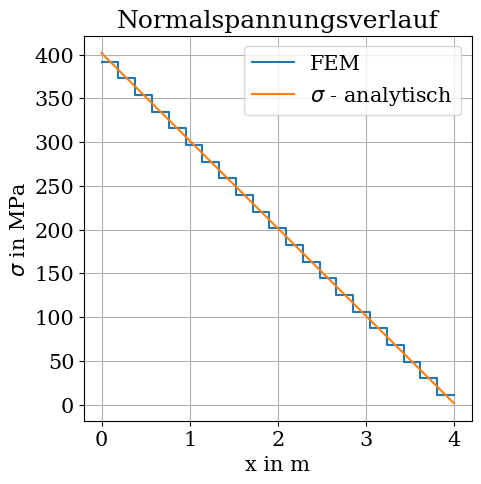
\includegraphics[width=0.75\linewidth]{files/Stab_Normalkraft_ref-092130b8e6ecfe32c195825bcc7079b4.png}
\caption[]{Ergebnisse für die Normalspannung in einem Stab unter Eigengewicht mit einer erhöhten Netzfeinheit.}
\label{stabelement_refined}
\end{figure}

Bei einer immer feiner werdenden Diskretisierung des Stabes konvergiert die Lösung gegen die analytische Lösung. Dennoch liegen, wie in Abbildung Figure~\ref{stabelement_refined} zu sehen, immer noch Spannungssprünge an den Elementgrenzen vor. Betrachtet man die Fehler der Spannungsergebnisse, so zeigt sich, dass dieser Fehler mit steigender Anzahl an Freiheitsgraden abnimmt. Dies ist in Abbildung Figure~\ref{stabelement_error} zu sehen. Im doppelt logarithmischen Ma$\beta$stab erhält man eine Gerade für die Abnahme des Fehlers. Auch bei der Verwendung von Ansatzfunktionen höherer Ordnung reduziert sich der Fehler nur linear im doppelt logarithmischen Ma$\beta$stab. Die Steigung ist jedoch höher, sodass im Allgemeinen mit einer verbesserten Konvergenz zu rechnen ist.

\begin{figure}[!htbp]
\centering
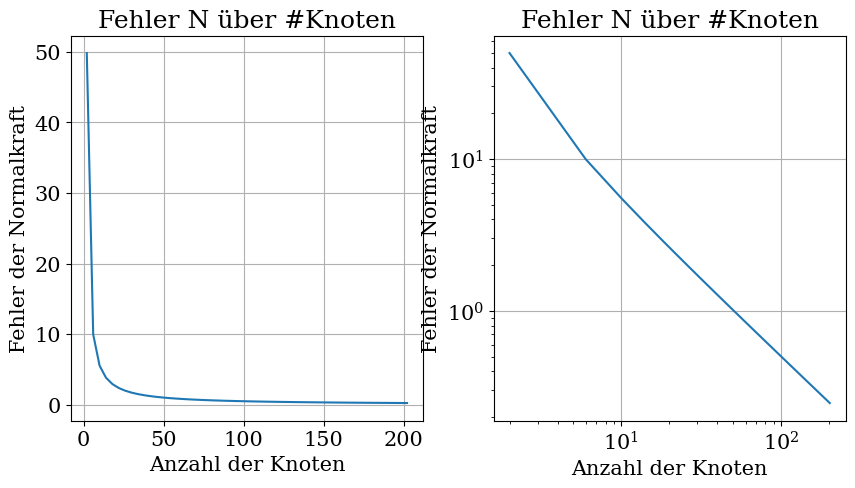
\includegraphics[width=0.75\linewidth]{files/Stab_error_convergen-416e1c43fb4900af48fee79e64009d70.png}
\caption[]{Konvergenz der Spannungsergebnisse in einem Stab unter Eigengewicht mit steigender Anzahl an Freiheitsgraden.}
\label{stabelement_error}
\end{figure}

\paragraph{Interaktives Notebook}

Basierend auf der präsentierten Theorie wurde ein Jupyter Notebook erstellt. Dieses kann man ohne Systemvoraussetzungen im Browser ausführen:

StabFEM for Binder: \href{https://mybinder.org/v2/gh/steffenbeese/FEM\_I\_Notebooks/main?urlpath=\%2Fdoc\%2Ftree\%2FNotebook\_StabFEM.ipynb}{
\includegraphics[width=0.2\linewidth]{files/b77199e99a54e59b2e3c037c2cc90f21.pdf}
}

\begin{framed}
\textbf{Fragen zum Kapitel}\\
\textbf{StabFEM}

\begin{itemize}
\item Was unterscheidet das Verfahren von Ritz von der FEM?
\item Welches Problem hat man beim Verfahren von Ritz bezüglich der Ansatzfunktion?
\item Skizzieren Sie die Formfunktionen für ein lineares Stabelement mit 2 Knoten.
\item Auf Elementebene werden die Steifigkeitsmatrizen und die Lastvektoren berechnet. Was passiert danach mit diesen Grö$\beta$en?
\item Das globale Gleichungssystem kann nicht gelöst werden. Die Steifigkeitsmatrix ist singulär. Was könnte der Grund dafür sein?
\end{itemize}
\end{framed}